\documentclass{fefu}
\usepackage{lipsum}

\usepackage{amssymb}
\usepackage{amsmath}
\usepackage{mathtools}
\usepackage{tikz}
\usepackage{array}
\usepackage{subcaption}
\usepackage{arydshln}
\usepackage{multirow}
\usepackage{minted}
\usepackage{tcolorbox}
\usepackage{graphicx}
\usepackage[toc,acronym,nonumberlist]{glossaries}

\graphicspath{{images/}}
\captionsetup[sub]{font=normalfont}

\newcommand{\pa}[1]{\left(#1\right)}
\newcommand{\param}[2]{%
    \textsf{#1} & #2\\
    \hline
}
\newcommand\rottext[2]{\rotatebox{90}{\parbox{#2}{\centering#1}}}
\newcommand{\PreserveBackslash}[1]{\let\temp=\\#1\let\\=\temp}
\newcolumntype{C}[1]{>{\PreserveBackslash\centering}p{#1}}

\makeatletter
\renewcommand\@biblabel[1]{\indent[#1]}
\makeatother

\usetikzlibrary{calc}
\usetikzlibrary{positioning}
\def\centerarc[#1](#2)(#3:#4:#5){ \draw[#1] ($(#2)+({#5*cos(#3)},{#5*sin(#3)})$) arc (#3:#4:#5) }
\tikzstyle{node} = [draw, fill=black, circle, inner sep=0pt, minimum height=2mm, minimum width=2mm]

\newglossarystyle{mystyle}{%
    \glsnogroupskiptrue%
    \renewenvironment{theglossary}{}{}%
    \renewcommand*{\glossentry}[2]{%
        \glsentryitem{##1}\textbf{\glstarget{##1}{\glossentryname{##1}}}~---~\glossentrydesc{##1}.\par
    }%
}
\setglossarystyle{mystyle}

\makeglossaries

\newglossaryentry{convex_hull}{name={Выпуклая оболочка},description={наименьшее  выпуклое множество, содержащее некоторое множество точек $X$}}

\newglossaryentry{tri_area}{name={Знаковая площадь треугольника},description={величина равная площади $S$ этого треугольника, если его вершины обходятся против часовой стрелки, и $-S$, если вершины упорядочены по часовой стрелке}}

\newglossaryentry{aperture}{name={Апертура},description={величина, определяющая максимальный угол отклонения лучей, от основого направления распространения}}

\newglossaryentry{triangulation}{name={Триангуляция},description={разбиение выпуклой оболочки множества точек $P$ на треугольники так, что любые два треугольника пересекаются в общей грани ребра или вершины, или вообще не пересекаются, и множество точек, являющиеся вершинами треульников разбиения, совпадает с $P$}}

\newacronym{MPE}{МПУ}{Модовое Параболическое Уравнение}
\newacronym{NAMPE}{УМПУ}{Узкоугольное Модовое Параболическое Уравнение}
\newacronym{WAMPE}{ШМПУ}{Широкоугольное Модовое Параболическое Уравнение}

\setglossarysection{subsubsection}

\begin{document}
    \setcounter{page}{2}
    \maketableofcontents
    \begin{abstract}
        \par Целью работы является вывод широкоугольного модового параболического уравнения из уравнения горизонтальной рефракции, используя рационально-линейную аппроксимацию оператора квадратного корня \cite{jensen}. В работе предложена конечно-разностная схема численного решения полученного уравнения. Схема основана на стандартном методе Крэнка-Николсон \cite{crank} и полностью дискретных условиях прозрачной границы, которые позволяют выполнять корректное моделирование распространения звука в неограниченной горизонтальной области. На основе полученной численной схемы разработана программа на языке программирования C++ \cite{c++}, использующая пакет Cambala \cite{cambala} для решения спектральной акустической задачи. Выполнен анализ корректности численной схемы и область её область применения на примере моделирования распространения в различных волноводах мелкого моря: волновод Пекериса, волноводы с подводным каньоном и клином.
    \end{abstract}
    \section{Введение}
        \subsection{Глоссарий}
            \printglossary[numberedsection,title=Термины]
              \printglossary[numberedsection,type=\acronymtype,title=Сокращения]
        \subsection{Описание предметной области}
            \subsubsection{Модовое представление звукового поля точечного источника}
                \paragraph{Модовые функции и волновые числа}
                    \par Звуковое поле $p\pa{x,y,z}$ (где $z$ обозначает глубину, а  $x,y$ --- координаты горизонтальной плоскости), создаваемое точечным источником в трёхмерном волноводе мелкого моря, расположенным по координатам $x=y=0$, $z=z_s$ и имеющего частоту $f$, описывается трёхмерным уравнением Гельмгольца \cite{jensen}
                    \begin{equation}\label{eq::3DH}
                        \pa{\rho\pa{z}\nabla\cdot\pa{\frac{1}{\rho\pa{z}}\nabla} + K\pa{z}^2}p\pa{x,y,z}=-\delta\pa{x}\delta\pa{y}\delta\pa{z-z_s}
                    \end{equation}
                    где $\rho\pa{z}$ --- плотность среды. Коэффициент $K\pa{z}$ определяется двумя способами:
                    \begin{enumerate}
                        \item Без учёта затухания:
                            \begin{equation}\label{eq::K1}
                                K\pa{z}=\frac{\omega}{c\pa{z}}\,,
                            \end{equation}
                        \item С учётом затухания:
                            \begin{equation}\label{eq::K2}
                                K\pa{z}=\frac{\omega}{c\pa{z}}\pa{1+i\eta\beta}\,,
                            \end{equation}
                    \end{enumerate}
                    где $c\pa{z}$ --- скорость звука, $\omega=2\pi f$ --- циклическая частота, $\beta$ --- коэффициент затухания, $\eta=\frac{1}{40\pi\log_{10}e}$. Используя технику разделения переменных и представляя звуковое поле в виде
                    \begin{equation}
                        p\pa{x,y,z}=A\pa{x,y}\varphi\pa{z}\,,
                    \end{equation}
                    при $x^2+y^2>0$ и $z\ne z_s$ уравнение \eqref{eq::3DH} можно привести к виду
                    \begin{multline}\label{eq::Sep3DH}
                        \frac{1}{A\pa{x,y}}\pa{\frac{\partial^2 A\pa{x,y}}{\partial x^2}+\frac{\partial^2 A\pa{x,y}}{\partial y^2}}+\\
                        \frac{1}{\varphi\pa{z}}\pa{\rho\pa{z}\frac{\partial}{\partial z}\pa{\frac{1}{\rho\pa{z}}\frac{\partial\varphi\pa{z}}{\partial z}}+K^2\varphi\pa{z}}=0\,.
                    \end{multline}
                    Вводя константу разделения $k_j^2$, из \eqref{eq::Sep3DH} можно получить модовое уравнение
                    \begin{equation}\label{eq::modal_equation}
                        \rho\pa{z}\frac{\partial}{\partial z}\pa{\frac{1}{\rho\pa{z}}\frac{\partial\varphi_j\pa{z}}{\partial z}}+\pa{K^2-k_j^2}\varphi_j\pa{z}=0\,.
                    \end{equation}
                    с граничными условиями на $z=0$ и $z=z_b$ ($z_b$ --- глубина дна). Функция $\varphi_j\pa{z}$ называется модовой функцией, а $k_j$ соответствующим ей волновым числом. Такое уравнение является классической задачей Штурма-Лиувилля, обладающая следующими свойствами:
                    \begin{enumerate}
                        \item модовое уравнение имеет бесконечное количество решений --- мод,
                        \item каждая такая мода характеризуется модовой функцией $\varphi_j\pa{z}$ и волновым числом $k_j$,
                        \item все $k_j$ различны,
                        \item функции $\varphi_j\pa{z}$ имеет ровно $j$ корней на отрезке $\left[0,z_b\right]$,
                        \item волновые числа удовлетворяют неравенству $k_1^2>k_2^2>k_3^2>\dots$,
                        \item без учёта затухания все волновые числа вещественны числа, с учётом --- комплексные,
                        \item модовые функции ортогональны и нормированы:
                            \begin{equation}
                                \int\limits_{0}^{z_b}\frac{\varphi_i\pa{z}\varphi_j\pa{z}}{\rho\pa{z}}\text{d}z=\delta_{ij},
                            \end{equation}
                        \item\label{complete_mode_set} модовые функции образуют полную систему.
                    \end{enumerate}
                    Используя \ref{complete_mode_set}, звуковое поле $p\pa{x,y,z}$ может быть представлено в виде модового разложения
                    \begin{equation}\label{eq::modal_decomposition}
                        p\pa{x,y,z}=\sum\limits_{j=1}^\infty A_j\pa{x,y}\varphi_j\pa{z}\,.
                    \end{equation}
                \paragraph{Случай горизонтальных неоднородностей среды}
                    \par В случае наличия горизонтальных неоднородностей среды вместо модового уравнения \eqref{eq::modal_equation} рассматривается модовое уравнение 
                    \begin{multline}\label{eq::ranged_modal_equation}
                        \rho\pa{z,x,y}\frac{\partial}{\partial z}\pa{\frac{1}{\rho\pa{z,x,y}}\frac{\partial\varphi_j\pa{z,x,y}}{\partial z}}+\\
                        \pa{K\pa{z,x,y}^2+k_j^2\pa{x,y}}\varphi_j\pa{z,x,y}=0\,.
                    \end{multline}
                    Таким образом, при любой фиксированной паре координат $x$, $y$ модовоые функции $\varphi_j\pa{z,x,y}$ и волновые числа $k_j\pa{x,y}$ находятся из решения уравнения \eqref{eq::ranged_modal_equation} с параметрами среды при этих горизонтальных координатах и обладают всеми свойствами мод, рассмотренных в случае горизонтально однородной среды. 
                \paragraph{Уравнение горизонтальной рефракции}
                    \par Рассматривается следующее уравнение Гельмгольца
                    \begin{equation}\label{eq::ranged_3DH}
                        \pa{\rho\pa{z}\nabla\cdot\pa{\frac{1}{\rho\pa{z}}\nabla} + K^2\pa{z,x,y}}p\pa{x,y,z}=-\delta\pa{x}\delta\pa{y}\delta\pa{z-z_s}\,,
                    \end{equation}
                    решение которого ищется в форме модового разложения 
                    \begin{equation}\label{eq::randed_modal_decompostion}
                        p\pa{x,y,z}=\sum\limits_{j=1}^\infty A_j\pa{x,y}\varphi_j\pa{z,x,y}\,.
                    \end{equation}
                    С учётом \eqref{eq::randed_modal_decompostion} уравнение \eqref{eq::ranged_3DH} преобразуется к виду
                    \begin{multline}\label{eq::modal_3DH}
                        \sum\limits_{j=1}^\infty\biggl[2\pa{\frac{\partial A_j\pa{x,y}}{\partial x}\frac{\partial\varphi_j\pa{z,x,y}}{\partial x}+\frac{\partial A_j\pa{x,y}}{\partial y}\frac{\partial\varphi_j\pa{z,x,y}}{\partial y}}\biggr]+\\
                        A_j\pa{x,y}\pa{\rho\pa{z}\frac{\partial}{\partial z}\pa{\frac{1}{\rho\pa{z}}\frac{\partial\varphi_j\pa{z,x,y}}{\partial z}}+K^2\pa{z,x,y}\varphi_j\pa{z,x,y}}+\\
                        \varphi_j\pa{z,x,y}\pa{\frac{\partial^2A_j\pa{x,y}}{\partial x^2}+\frac{\partial^2A_j\pa{x,y}}{\partial y^2}}=-\delta\pa{x}\delta\pa{y}\delta\pa{z-z_s}\,.
                    \end{multline}
                    Учитывая \eqref{eq::ranged_modal_equation}, применяя оператор
                    \begin{equation}
                        \int\pa{\cdot}\frac{\varphi_j\pa{z,x,y}}{\rho\pa{z}}\text{d}z\,,
                    \end{equation}
                    используя свойства ортогональности модовых функций, и рассматривая конкретное $j$, уравнение \eqref{eq::modal_3DH} можно привести к виду
                    \begin{multline}
                        \frac{\partial^2A_j\pa{x,y}}{\partial x^2}+\frac{\partial^2A_j\pa{x,y}}{\partial y^2}+k_j^2\pa{x,y}A_j\pa{x,y}+\\
                        \sum\limits_{i=1}^\infty\left[\alpha_{ij}A_i\pa{x,y}+2\pa{\beta_{ij}\frac{\partial A_i\pa{x,y}}{\partial x}+\gamma_{ij}\frac{\partial A_i\pa{x,y}}{\partial y}}\right]=-\delta\pa{x}\delta\pa{y}\delta\pa{z-z_s}\,,
                    \end{multline}
                    где
                    \begin{equation}
                        \begin{aligned}
                            \alpha_{ij}&=\int\pa{\frac{\partial}{\partial x}+\frac{\partial}{\partial y}}\frac{\varphi_i\pa{z,x,y}\varphi_j\pa{z,x,y}}{\rho\pa{z}}\text{d}z\,,\\
                            \beta_{ij}&=-\beta_{ji}=\int\frac{\partial\varphi_i\pa{z,x,y}}{\partial x}\frac{\varphi_j\pa{z,x,y}}{\rho\pa{z}}\text{d}z\,,\\
                            \gamma_{ij}&=-\gamma_{ji}=\int\frac{\partial\varphi_i\pa{z,x,y}}{\partial y}\frac{\varphi_j\pa{z,x,y}}{\rho\pa{z}}\text{d}z\,.
                        \end{aligned}
                    \end{equation}
                    Коэффициенты $\alpha_{ij}$, $\beta_{ij}$, $\gamma_{ij}$ отвечают за межмодовое взаимодействие. Получаемая пренебрежением этим взаимодействием адиабатическая аппроксимация даёт уравнение горизонтальной рефракции
                    \begin{equation}\label{eq::HRE}
                        \pa{\Delta+k_j^2\pa{x,y}}A_j\pa{x,y}=-\varphi_j\pa{z_s}\delta\pa{x}\delta\pa{y}\,.
                    \end{equation}
                    Функции $A_j\pa{x,y}$ называются модовыми амплитудами. Модовые функции\\ $\varphi_j\pa{z,x,y}$ и соответствующие им горизонтальные волновые числа $k_j\pa{x,y}$ находятся из решения соответствующей акустической спектральной задачи \eqref{eq::ranged_modal_equation}.
            \subsubsection{Модовые параболические уравнения}
                \par Для решения уравнения горизонтальной рефракции было разработано множество методов с момента его появления в 1970х годах: акустическая лучевая теория \cite{burridge}, параболические аппроксимации \cite{collins} и различные специальные методы (например \cite{petrov14}).
                \par В данной работе подробно рассматриваются параболические аппроксимации уравнения горизонтальной рефракции, называемые модовыми параболическими уравнениями, которые впервые были введены М. Д. Коллинзом в 1993 году \cite{collins}. Вообще говоря, такое уравнение может быть решено точно такими же методами, что уравнение Шрёдингера и параболические (параксиальные) уравнения в оптике и радиофизике: конечные разности, экспоненциальная временная разность, метод Фурье разделённого шага и многие другие \cite{jensen}. В некоторых особенных случаях МПУ также имеет аналитическое решение с использованием теории групп \cite{petrov16, petrov17}. 
                \paragraph{\label{sec::PDMPE}Псевдо-дифференциальное МПУ}
                    \par Для получения параболических аппроксимаций уравнения горизонтальной рефракции в первую очень необходимо вывести псевдо-дифференциальное модовое параболическое уравнение. Для этого \eqref{eq::HRE} представляется в виде
                    \begin{equation}
                        \pa{\frac{\partial}{\partial x}+i\sqrt{k_j^2\pa{x,y}+\frac{\partial^2}{\partial z^2}}}\pa{\frac{\partial}{\partial x}-i\sqrt{k_j^2\pa{x,y}+\frac{\partial^2}{\partial z^2}}}A_j\pa{x,y}=0\,,
                    \end{equation}
                    и выделяется его решение, состоящее из волн, распространяющихся в положительном направлении оси $x$
                    \begin{equation}
                        \pa{\frac{\partial}{\partial x}-i\sqrt{k_j^2\pa{x,y}+\frac{\partial^2}{\partial z^2}}}A_j\pa{x,y}=0\,.
                    \end{equation}
                    Вводя модовое опорное волновое число $k_{j,0}$ и выделяя главную осцилляцию из $A_j\pa{x,y}$
                    \begin{equation*}
                        A_j\pa{x,y}=e^{k_{j,0}x}\mathcal{A}_j\pa{x,y}\,,
                    \end{equation*}
                    получим псевдо-дифференциальное модовое параболическое уравнение
                    \begin{equation}\label{eq::PDMPE}
                        \frac{\partial\mathcal{A}_j\pa{x,y}}{\partial x}=ik_{j,0}\pa{\sqrt{1+L_j}-1}\mathcal{A}_j\pa{x,y}\,,
                    \end{equation}
                    где 
                    \begin{equation*}
                        k_{j,0}^2L_j=\frac{\partial^2}{\partial z^2}+k_j^2\pa{x,y}-k_{j,0}^2\,.
                    \end{equation*}
                    Это уравнение является эволюционным по координате $x$ и представляет собой однонаправленное волновое уравнение ($x$ обозначает <<время>>, $y$ --- <<пространство>>). Также оно является основой для получения различных форм параболических аппроксимаций, представляющих собой уравнения в частных производных первого порядка по переменной $x$, которые определяются видом аппроксимации псевдо-дифференциального оператора квадратного корня $\sqrt{1+L_j}$ \cite{jensen}.
                \paragraph{Узкоугольное МПУ}
                    \par Простейшей такой аппроксимацией является приближение Тапперта \cite{jensen}
                    \begin{equation}\label{eq::tappert}
                        \sqrt{1+L_j}\simeq 1+\frac{L_j}{2}\,,
                    \end{equation}
                    которое представляет собой первые два члена разложения оператора в ряд Тейлора. С использованием \eqref{eq::tappert} получим стандартное узкоугольное модовое параболическое уравнение из \eqref{eq::PDMPE}
                    \begin{equation}
                        \frac{\partial\mathcal{A}_j\pa{x,y}}{\partial x}=\frac{ik_{j,0}L_j}{2}\mathcal{A}_j\pa{x,y}
                    \end{equation}
                    или
                    \begin{equation}\label{eq::NAMPE}
                        2ik_{j,0}\frac{\partial\mathcal{A}_j\pa{x,y}}{\partial x}+\frac{\partial^2\mathcal{A}_j\pa{x,y}}{\partial y^2}+\pa{k_j^2\pa{x,y}-k_{j,0}^2}\mathcal{A}_j\pa{x,y}=0\,.
                    \end{equation}
                    Такое уравнение считается корректным для моделирования распространения волн под углом $\pm 10\text{--}15^\circ$ от направления распространения. В качестве начального условия при $x=0$ для решения УМПУ используется функция Гаусса:
                    \begin{equation}\label{eq::gaussian_function}
                        \mathcal{A}_j\pa{0,y}=\frac{\varphi_j\pa{z_s}}{2\sqrt{\pi}}e^{-k_{j,0}^2y^2}\,.
                    \end{equation}
                    \par Несмотря на то, что УМПУ получило широкое распространение, для многих задач требуется учёт волн, распространяющихся под большими углами, которые не могут быть учтены в рамках данной модели, поэтому возникает необходимость в широкоугольных модовых параболических уравнениях.
                \paragraph{Широкоугольное МПУ}
                    \par Для того, чтобы получить широкоугольное модовое параболическое уравнение, используется рационально-линейная функция
                    \begin{equation}\label{eq::rational_linear}
                        \sqrt{1+L_j}\simeq\frac{a+bL_j}{1+cL_j}\,,
                    \end{equation}
                    где $a$, $b$, $c$ --- определённые константы, выбор которых подробно описан в \cite{jensen}. Заменяя \eqref{eq::rational_linear} в \eqref{eq::PDMPE}, получим
                    \begin{equation}\label{eq::almost_WAMPE}
                        \frac{\partial\mathcal{A}_j\pa{x,y}}{\partial x}=ik_{j,0}\pa{\frac{a+bL_j}{1+cL_j}-1}\mathcal{A}_j\pa{x,y}\,.
                    \end{equation}
                    Вводя обозначения $\alpha_0=a-1$, $\alpha_1=b-c$, преобразуем \eqref{eq::almost_WAMPE} в следующее широкоугольное модовое параболическое уравнение
                    \begin{equation}\label{eq::WAMPE}
                        \frac{\partial\mathcal{A}_j\pa{x,y}}{\partial x}=ik_{j,0}\frac{\alpha_0+\alpha_1L_j}{1+cL_j}\mathcal{A}_j\pa{x,y}\,.
                    \end{equation}
                    Таким образом, использование более точной аппроксимации оператора квадратного корня $\sqrt{1+L_j}$ позволяет получить уравнение, корректно моделирующие распространение волн под углом $\pm40^\circ$ к основному направлению распространения. Функция Гаусса \eqref{eq::gaussian_function}, используемая в качестве начального условия для УМПУ, не соответствует широкоугольным свойствам новой модели, что отрицательно сказывается на точности вычисляемого решения, поэтому в качестве начального условия при $x=0$ необходимо использовать широкоугольные функции. Примером такой функции является так называемый источник Грина \cite{jensen}
                    \begin{equation}\label{eq::greene_function}
                        \mathcal{A}_j\pa{0,y}=\frac{\varphi_j\pa{z_s}}{2\sqrt{\pi}}\pa{1.4467-0.8402k_{j,0}^2y^2}e^{-\frac{k_{j,0}^2y^2}{1.5256}}\,.
                    \end{equation}
                    \par Несмотря на то, что полученное уравнение имеет лучшие свойства по сравнению с УМПУ, оно не получило широкого распространения и было плохо изучено, хотя стандартные широкоугольные параболические уравнения, решаемые в вертикальной плоскости, часто используются в подводной акустике \cite{claerbout,jensen,greene}. Также следует заметить, что при $a=1$, $b=1/2$, $c=0$ широкоугольное уравнение \eqref{eq::WAMPE} становится узкоугольным уравнением \eqref{eq::NAMPE}.
                \paragraph{Очень широкоугольное МПУ}
                    \par Существует также класс очень широкоугольных параболических уравнений, получаемых при использовании нескольких членов разложения оператора квадратного корня в ряд, например, аппроксимация Паде \cite{jensen}
                    \begin{equation}
                        \sqrt{1+L_j}=1+\sum\limits_{k=1}^m\frac{a_{k,m}L_j}{1+b_{k,m}L_j}+O\pa{q^{2m+1}}\,,
                    \end{equation}
                    где коэффициенты определяются как
                    \begin{align*}
                        a_{k,m}&=\frac{2}{2m+1}\sin^2\pa{\frac{k\pi}{2m+1}}\,,\\
                        b_{k,m}&=\cos^2\pa{\frac{k\pi}{2m+1}}\,.
                    \end{align*}
                    Полученное таким образом очень широкоугольное модовое параболическое уравнение имеет вид
                    \begin{equation}
                        \frac{\partial\mathcal{A}_j\pa{x,y}}{\partial x}=ik_{j,0}\pa{\sum\limits_{k=1}^m\frac{a_{k,m}L_j}{1+b_{k,m}L_j}}\mathcal{A}_j\pa{x,y}\,.
                    \end{equation}
                    Использование большого количества членов ряда позволяет учитывать почти полный $\pm90^{\circ}$ спектр распространяющихся волн. Однако поиск решения такого уравнения влечёт огромные вычислительные затраты, поэтому изучение обычного широкоугольного параболического уравнения и области его применения является более приоритетной задачей.
        \subsection{Неформальная постановка задачи}
            \par В рамкам данной работы необходимо выполнить следующие задачи:
            \begin{enumerate}
                \item Исследовать особенности методов решения МПУ, в том числе применение условий прозрачной границы;
                \item Разработать численную схему решения ШМПУ с использованием полностью дискретных условий прозрачной границы;
                \item Разработать комплекс программ для вычисления звукового поля точечного источника в мелком море с использованием модового разложения, эффективно реализующий полученную численную схему;
                \item Включить в алгоритм вычисления решения ШМПУ расчёт коэффициентов уравнения путём решения акустической спектральной задачи с использованием пакета Cambala \cite{cambala};
                \item Изучить область применения ШМПУ и корректность численной схемы его решения.
            \end{enumerate}
            \subsubsection{Требования к программной реализации}
                \par Известные математические пакеты и библиотеки не предоставляют возможности использования условий прозрачной границы, поэтому возникает задача разработки новой программы. Основными требования к которой являются:
                \begin{enumerate}
                    \item Возможность использования как готовых коэффициентов уравнения, так и коэффициентов, вычисленных с помощью пакета Cambala, с указанием необходимых параметров среды: плотности среды, батиметрия, гидрология и др.;
                    \item Возможность сохранения вычисленных коэффициентов уравнения;
                    \item Высокая скорость работы и низкая потребность в памяти.
                \end{enumerate}
        \subsection{Обзор существующих методов решения}
            \par Для решения уравнения Гельмгольца \eqref{eq::3DH} были разработаны различные методы: трассировка модовых гауссовых лучей \cite{trofimov16}, решение трёхмерного модового параболического уравнения \cite{isakson14,lin12,shtrum16}, метод мнимых источников \cite{deane93, tang18}. Такие методы требуют огромных вычислительных затрат (время вычисления часто составляет несколько часов или дней), однако они подходят для решения широко класса задач и имеют высокую точность, поэтому часто используются в качестве эталонных решений при разработке новых методов. Также известны методы, основанные на узкоугольных параболических уравнениях с учётом взаимодействия мод \cite{trofimov15} и без \cite{petrov16}, но, как было сказано ранее, такие методы имеют ограниченную область применения. Поэтому возникает необходимость в разработке новых моделей и методов, имеющих большую область применения, но требующих небольших вычислительных затрат.
        \subsection{План работ}
            \begin{enumerate}
                \item Исследование методов решения МПУ и условий прозрачной границы;
                \item Разработка численной схемы решения ШМПУ с применением полностью дискретных условий прозрачной границы;
                \item Разработка программы, реализующей полученную численную схему;
                \item Добавление использования пакета Cambala в разарботанную программу для решения акустической спектральной задачи;
                \item Изучение корректности полученной численной схемы и области её применения, тестирование программы.
            \end{enumerate}
        \subsection{Математические методы}
            \subsubsection{Математическая постановка задачи\label{sec::MPD}}
                \par Необходимо в области $\Omega=\left\{\pa{x,y,z}\big|0\leqslant x\leqslant x_1,y_0\leqslant y\leqslant y_1,0\leqslant z\leqslant z_b\right\}$ найти звуковое поле $p\pa{x,y,z}$ точечного источника, являющееся решением уравнения Гельмгольца
                \begin{multline}
                    \frac{\partial^2p\pa{x,y,z}}{\partial x^2}+\frac{\partial^2p\pa{x,y,z}}{\partial y^2}+\rho\pa{z}\frac{\partial}{\partial z}\pa{\frac{1}{\rho\pa{z}}\frac{\partial p\pa{x,y,z}}{\partial z}}+\\
                    K^2\pa{z,x}p\pa{x,y,z}=-\delta\pa{x}\delta\pa{y}\delta\pa{z-z_s}\,,
                \end{multline}
                в форме модового разложения
                \begin{equation}
                    p\pa{x,y,z}=\sum\limits_{j=1}^Je^{k_{j,0}x}\mathcal{A}_j\pa{x,y}\varphi_j\pa{z,x,y}\,.
                \end{equation}
                наблюдаемого приёмником, расположенным на глубине $z_r$. Модовые амплитуды $\mathcal{A}_j\pa{x,y}$ являются решениями соответствующих задач Коши
                \begin{equation}\label{eq::WAMPE_problem}
                    \begin{dcases}
                        \frac{\partial\mathcal{A}_j\pa{x,y}}{\partial x}=ik_{j,0}\frac{\alpha_0+\alpha_1L_j}{1+cL_j}\mathcal{A}_j\pa{x,y}\,,\\
                        \mathcal{A}_j\pa{0,y}=\frac{\varphi_j\pa{z_s}}{2\sqrt{\pi}}\pa{1.4467-0.8402k_{j,0}^2y^2}e^{-\frac{k_{j,0}^2y^2}{1.5256}}\,.
                    \end{dcases}
                \end{equation}
                При этом считается, что модововые функции $\varphi_j\pa{z,x,y}$ и соответствующие им волновые числа $k_j\pa{x,y}$ заранее известны из решения спектральной задачи \eqref{eq::ranged_modal_equation}.
            \subsubsection{Метод Крэнка-Николсон}
                \par Метод Крэнка-Николсон является методом конечных разностей, разработанный для численного решения решения уравнения теплопроводности и схожих уравнений в частных производных. Метод был разработан Джоном Крэнком и Филлис Николсон в середине 20-го века \cite{crank}. Метод основан на методе трапеций решения дифференциальных уравнений, вычислительно стабилен, имеет второй порядок точности по переменной <<времени>> и является неявным по ней. 
                \par Пусть задано уравнение вида
                \begin{equation}
                    \frac{\partial u}{\partial t}=F\pa{u,x,t,\frac{\partial u}{\partial x}, \frac{\partial^2u}{\partial x^2}}\,.
                \end{equation}
                Тогда, считая $u\pa{i\Delta x, j\Delta t}=u_{i,j}$, метод Крэнка-Николсон можно записать как комбинацию прямого метода Эйлера на шаге $j$
                \begin{equation}
                    \frac{u_{i,j+1}-u_{i,j}}{\Delta t}=F_{i,j}\pa{u,x,t,\frac{\partial u}{\partial x},\frac{\partial^2u}{\partial x^2}}
                \end{equation}
                и обратного метода Эйлера на шаге $j+1$
                \begin{equation}
                    \frac{u_{i,j+1}-u_{i,j}}{\Delta t}=F_{i,j+1}\pa{u,x,t,\frac{\partial u}{\partial x},\frac{\partial^2u}{\partial x^2}}
                \end{equation}
                в виде
                \begin{equation}
                    \frac{u_{i,j+1}-u_{i,j}}{\Delta t}=\frac{1}{2}\left[F_{i,j+1}\pa{u,x,t,\frac{\partial u}{\partial x},\frac{\partial^2u}{\partial x^2}}+F_{i,j}\pa{u,x,t,\frac{\partial u}{\partial x},\frac{\partial^2u}{\partial x^2}}\right]\,.
                \end{equation}
                Следует заметить, что метод не является простым алгебраическим средним, так как обратный метод Эйлера имеет неявную зависимость от решения, поэтому и сам метод Крэнка-Николсон является неявным и требует вычисления решения системы алгебраических уравнений для получения <<следующего>> значения $u$ во времени. Такая система будет являться линейной, если исходное уравнение линейно, и нелинейной в противном случае. Схема метода Крэнка-Николсон при использовании конечных разностей второго порядка аппроксимации производных по переменной $x$ изображена на Рис. \ref{fig::CNS}.
                \begin{figure}[h]
                    \centering
                    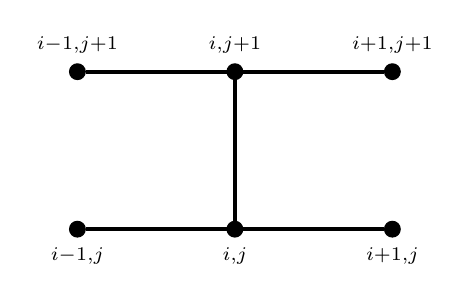
\begin{tikzpicture}[node distance=2cm]
                        \node[node, label=above:{$\scriptstyle{i-1,j+1}$}](N1) {};
                        \node[node, right of=N1, label=above:{$\scriptstyle{i,j+1}$}](N2) {};
                        \node[node, right of=N2, label=above:{$\scriptstyle{i+1,j+1}$}](N3) {};
                        \node[node, below of=N2, label=below:{$\scriptstyle{i,j}$}](N4) {};
                        \node[node, left of=N4, label=below:{$\scriptstyle{i-1,j}$}](N5) {};
                        \node[node, right of=N4, label=below:{$\scriptstyle{i+1,j}$}](N6) {};
        
                        \draw[-, line width=0.5mm] (N1) -- (N3);
                        \draw[-, line width=0.5mm] (N5) -- (N6);
                        \draw[-, line width=0.5mm] (N2) -- (N4);
                    \end{tikzpicture}
                    \caption{\label{fig::CNS}Схема метода Крэнка-Николсон}
                \end{figure}
            \subsubsection{\label{sec::numerical_scheme}Численная схема решения ШМПУ}
                \par В данной работе для решения задачи \eqref{eq::WAMPE_problem} была разработана численная схема, основанная на метод Крэнка-Николсон. Будем рассматривать следующую равномерную сетку
                \begin{equation}
                    \begin{aligned}
                        x_n&=n\Delta x\,,&n&=\overline{0,N}\,,\\
                        y_m&=y_0+m\Delta y\,,&m&=\overline{0,M}\,,\\
                        \Delta x&=\frac{x_1}{N-1}\,,&k_j^{n,m}&=k_j\pa{x_n,y_m}\,,\\
                        \Delta y&=\frac{y_1-y_0}{M-1}\,,&\mathcal{A}_j^{n,m}&\approx\mathcal{A}_j\pa{x_n,y_m}\,.
                    \end{aligned}
                \end{equation}
                Преобразовывая ШМПУ в \eqref{eq::WAMPE_problem} к виду
                \begin{equation}\label{eq::evolution_equation}
                    \pa{1+cL_j}\frac{\partial\mathcal{A}_j}{\partial x}=ik_{j,0}\pa{\alpha_0+\alpha_1L_j}\mathcal{A}_j
                \end{equation}
                и используя дискретизацию Крэнка-Николсон, получим следующее уравнение в конечных разностях:
                \begin{equation}
                    \pa{1+cL_j^{\frac{n}{2},m}}\frac{\mathcal{A}_j^{n+1,m}-\mathcal{A}_j^{n,m}}{\Delta x}=ik_{j,0}\pa{\alpha_0+\alpha_1L_j^{\frac{n}{2},m}}\frac{\mathcal{A}_j^{n+1,m}+\mathcal{A}_j^{n,m}}{2}\,,
                \end{equation}
                где 
                \begin{align*}
                    k_{j,0}^2L_j^{\frac{n}{2},m}&=\frac{\partial^2}{\partial y^2}+\kappa_j^{\frac{n}{2},m}-k_{j,0}^2\,,\\
                    \kappa_j^{\frac{n}{2},m}&=\frac{\pa{k_j^{n+1,m}}^2+\pa{k_j^{n,m}}^2}{2}\,.
                \end{align*}
                Объединяя члены с одинаковым $n$ и вводя коэффициенты
                \begin{align*}
                    \beta_{j,0}&=2-\alpha_0ik_{j,0}\Delta x\,,&\beta_{j,1}&=2c-\alpha_1ik_{j,0}\Delta x\,,\\
                    \gamma_{j,0}&=2+\alpha_0ik_{j,0}\Delta x\,,&\gamma_{j,1}&=2c+\alpha_1ik_{j,0}\Delta x\,,
                \end{align*}
                придём к маршевой численной схеме, которая аппроксимирует эволюционное уравнение \eqref{eq::evolution_equation}:
                \begin{equation}
                    \pa{\beta_{j,0}+\beta_{j,1}L_j^{\frac{n}{2},m}}\mathcal{A}_j^{n+1,m}=\pa{\gamma_{j,0}+\gamma_{j,1}L_j^{\frac{n}{2},m}}\mathcal{A}_j^{n,m}\,.
                \end{equation}
                Аппроксимируя дифференциальный оператор в $L_j^{\frac{n}{2},m}$ центральной разностью второго порядка
                \begin{equation}
                    \frac{\partial^2\mathcal{A}_j^{n,m}}{\partial y^2}\approx\frac{\mathcal{A}_j^{n,m+1}-2\mathcal{A}_j^{n,m}+\mathcal{A}_j^{n,m-1}}{\Delta y^2}\,,
                \end{equation}
                получим следующие дискретизированное ШМПУ:
                \begin{equation}
                    u_{j,0}\mathcal{A}_j^{n+1,m+1}+v_{j,0}^{n,m}\mathcal{A}_j^{n+1,m}+u_{j,0}\mathcal{A}_j^{n+1,m-1}=
                    u_{j,1}\mathcal{A}_j^{n,m+1}+v_{j,1}^{n,m}\mathcal{A}_j^{n,m}+p_{j,1}\mathcal{A}_j^{n,m-1}\,,
                \end{equation}
                где
                \begin{gather}
                    \begin{aligned}
                        u_{j,0}&=\frac{\beta_{j,1}}{k_{j,0}^2\Delta y^2}\,,&v_{j,0}^{n,m}&=\beta_{j,0}-\beta_{j,1}\mathcal{L}_j^{n,m}\,,\\
                        u_{j,1}&=\frac{\gamma_{j,1}}{k_{j,0}^2\Delta y^2}\,,&v_{j,1}^{n,m}&=\gamma_{j,0}-\gamma_{j,1}\mathcal{L}_j^{n,m}\,,
                    \end{aligned}\\
                    \mathcal{L}_{j}^{n,m}=\frac{1}{k_{j,0}^2}\pa{\kappa_j^{\frac{n}{2},m}-k_{j,0}^2-\frac{2}{\Delta y^2}}\,.
                \end{gather}
            \subsubsection{Условия прозрачной границы\label{sec::TBC}}
                \par Одной из особенностей МПУ является то, что их решение всегда рассматривается в неограниченной области, в отличие от решения <<обычных>>, или <<вертикальных>>, параболических уравнений в подводной акустике, которое вычисляется в нескольких слоях, имеющих в качестве верхней границы поверхность океана и, как минимум в теории, некоторую границу на дне моря. Таким образом, искусственное ограничение вычислительной области является обязательным при численном решении МПУ. На таких искусственных границах необходимо установить прозрачные или поглощающие условия. Такие условие были хорошо изучены для узкоугольных параболических уравнений \cite{baskakov,antoine}.
                \par Чтобы эмулировать вычисление решения ШМПУ в рамках данной работы было решено адаптировать полностью дискретные прозрачные граничные условия, изначально разработанные для <<вертикальных>> параболических уравнений A. Arnold и M. Ehrhardt в 1998 году \cite{arnold}. Условия ставятся на границах области при $y=y_0$ и $y=y_M$.
                \par Чтобы использовать эти граничные условия необходимо установить, что волновые числа $k_j$ являются постоянными на этих границах, то есть не зависят от переменной $x$, а среда в свою очередь является однородной:
                \begin{align}
                    \begin{array}{lllll}
                        k_j^{n,0}&=&k_j^0&=&k_j\pa{0,y_0}\,,\\
                        k_j^{n,M}&=&k_j^M&=&k_j\pa{0,y_M}\,,
                    \end{array}
                    &&\forall n=\overline{0,N}\,.&
                \end{align}
                Действительно, если на границе присутствуют неоднородности среди, то невозможно учесть волны отражённые обратно в вычислительную область от этих неоднородностей. 
                \par Полностью дискретные прозрачные граничные условия при $y=y_0$ записываются в виде
                \begin{equation}\label{eq::TBC}
                    \pa{1+iq_j}\mathcal{A}_j^{n+1,1}-s_{j,0}^{\pa{0}}\mathcal{A}_j^{n+1,0}=-\pa{1-iq_j}\mathcal{A}_j^{n,1}+\sum\limits_{l=1}^ns_{0,j}^{\pa{n-l+1}}\mathcal{A}_j^{l,0}\,,
                \end{equation}
                где $q_j=2c/\pa{k_{j,0}\alpha_1\Delta x}$. Коэффициенты $s_{j,0}^{\pa{l}}$ могут быть найдены по рекурсивной формуле \cite{arnold}:
                \begin{equation}\label{eq::SS}
                    \begin{aligned}
                        s_{j,0}^{\pa{0}}&=1+iq_j-\frac{i}{2}\pa{\gamma_j+i\sigma_j+\sqrt[+]{A_j}}\,,\\
                        s_{j,0}^{\pa{1}}&=1-iq_j+\frac{i}{2}\pa{\gamma_j-i\sigma_j+\frac{B_j}{\sqrt[+]{A_j}}}\,,\\
                        s_{j,0}^{\pa{2}}&=\frac{\mu_j}{2\lambda_j}\pa{s_{j,0}^{\pa{1}}+\frac{s_{j,0}^{\pa{0}}}{\lambda_j\mu_j}-\beta_j}\,,\\
                        s_{j,0}^{\pa{l+1}}&=\frac{1}{l+1}\pa{\frac{2l-1}{\lambda_j}\mu_js_{j,0}^{\pa{l}}-\frac{l-2}{\lambda_j^2}s_{j,0}^{\pa{l-1}}}\,,
                    \end{aligned}
                \end{equation}
                где
                \begin{gather}
                    R_j=\frac{2k_{j,0}}{\alpha_1}\frac{\Delta y^2}{\Delta x}\,,\qquad\delta_j=1-c\pa{1-N_{j,0}^2}\,,\nonumber\\
                    \kappa_j=\frac{\Delta xk_{j,0}}{2}\pa{\alpha_0-\alpha_1\pa{1-N_{j,0}^2}}\,,\nonumber\\
                    \gamma_j=R_j\delta_j\,,\qquad\sigma_j=-R_j\kappa_k\,,\qquad N_{j,0}=\frac{k_{j,0}}{k_j^0}\,,\nonumber\\
                    \lambda_j=\frac{\sqrt[+]{A_j}}{\sqrt[+]{C_j}}\,,\quad\mu_j=\frac{B_j}{\sqrt[+]{A_j}\sqrt[+]{C_j}}\,,\nonumber\\
                    \begin{aligned}
                        A_j&=\pa{\gamma_j-i\sigma_j}\pa{\gamma_j-4q_j+i\pa{\sigma_j+4}}\,,\\
                        B_j&=\gamma_j\pa{\gamma_j-4q_j}+\sigma_j\pa{\sigma_j+4}\,,\\
                        C_j&=\pa{\gamma_j-i\sigma_j}\pa{\gamma_j-4q_j-i\pa{\sigma_j+4}}\,,
                    \end{aligned}\nonumber\\
                    \beta=1-iq_j+\frac{i}{2}\pa{\gamma_j-i\sigma_j}+\frac{C_j}{B_j}\pa{1+iq_j-\frac{i}{2}\pa{\gamma_j+i\sigma_j}}\,.
                \end{gather}
                Здесь $\sqrt[+]{\pa{\cdot}}$ означает значение корня, вещественная часть которого положительна. При $y=y_M$ прозрачные граничные условия записываются в виде:
                \begin{equation}
                    \pa{1+iq_j}\mathcal{A}_j^{n+1,M-1}-s_{j,M}^{\pa{0}}\mathcal{A}_j^{n+1,M}=-\pa{1-iq_j}\mathcal{A}_j^{n,M-1}+\sum\limits_{l=1}^ns_{j,M}^{\pa{n-l-1}}\mathcal{A}_j^{l,M}\,.
                \end{equation}
                Коэффициенты $s_{j,M}^{\pa{l}}$ вычисляются аналогично \eqref{eq::SS}.
                \par Следует заметить, что в граничных условиях присутствует сумма по всем предыдущим значениям функции на границе, поэтому при большом количество точек по переменной $x$ вычисление этой суммы может стать очень затратным, поэтому можно учитывать только значения из <<недавнего прошлого>>, тогда условия примут вид:
                \begin{equation}\label{eq::TBCW}
                    \pa{1+iq_j}\mathcal{A}_j^{n+1,1}-s_{j,0}^{\pa{0}}\mathcal{A}_j^{n+1,0}=-\pa{1-iq_j}\mathcal{A}_j^{n,1}+\sum\limits_{l=\max\left\{1,n-W\right\}}^ns_{0,j}^{\pa{n-l+1}}\mathcal{A}_j^{l,0}\,,
                \end{equation}
                где $W$ --- количество учитываемых значений. Однако в таком случае может происходить отражение от границы, даже при достаточно больших $W$.
            \subsubsection{Вычислительная сложность численной схемы}
                \par Таким образом, вычисление решения ШМПУ с использованием полученной численной схемы состоит в решении системы из $M$ линейных алгебраических уравнений вида на каждом шаге $n$ по переменной $x$ для каждой моды $j$:
                \begin{equation}
                    \begin{dcases}
                        \pa{1+iq_j}\mathcal{A}_j^{n+1,1}-s_{j,0}^{\pa{0}}\mathcal{A}_j^{n+1,0}=-\pa{1-iq_j}\mathcal{A}_j^{n,1}+\sum\limits_{l=1}^ns_{0,j}^{\pa{n-l+1}}\mathcal{A}_j^{l,0}\,,\\
                        \dots\\
                        u_{j,0}\mathcal{A}_j^{n+1,m+1}+v_{j,0}^{n,m}\mathcal{A}_j^{n+1,m}+u_{j,0}\mathcal{A}_j^{n+1,m-1}=\\
                        \kern6cm u_{j,1}\mathcal{A}_j^{n,m+1}+v_{j,1}^{n,m}\mathcal{A}_j^{n,m}+p_{j,1}\mathcal{A}_j^{n,m-1}\,,\\
                        \dots\\
                        \pa{1+iq_j}\mathcal{A}_j^{n+1,M-1}-s_{j,M}^{\pa{0}}\mathcal{A}_j^{n+1,M}=-\pa{1-iq_j}\mathcal{A}_j^{n,M-1}+\sum\limits_{l=1}^ns_{j,M}^{\pa{n-l-1}}\mathcal{A}_j^{l,M}
                    \end{dcases}
                \end{equation}
                Матрица такой системы является трёхдиагональной
                \vspace{-0.3cm}
                \begin{equation}
                    \begin{pmatrix}
                        -s_{j,0}^{\pa{0}} & 1+iq_j & 0 & 0 & 0 & 0 & 0 & \dots & 0\\
                        \vdots & \ddots & \vdots & \vdots & \vdots & \vdots & \vdots & \ddots & \vdots\\
                        0 & \dots & 0 & u_{j,0} & v_{j,0}^{n,m} & u_{j,0} & 0 & \dots & 0\\
                        \vdots & \ddots & \vdots & \vdots & \vdots & \vdots & \vdots & \ddots & \vdots\\
                        0 & \dots & 0 & 0 & 0 & 0 & 0 & 1+iq_j & -s_{j,M}^{\pa{0}} 
                    \end{pmatrix}
                \end{equation}
                поэтому система может быть решена методом прогонки \cite{abramov}.
                \par Таким образом вычислительная сложность алгоритма составляет $O\pa{JN^2M}$, где $J$ --- количество учитываемых мод. Так как используемая модель не учитывает межмодовое взаимодействие, уравнение для каждой отдельной моды не зависит от остальных, поэтому полученный алгоритм может быть эффективно реализован с использованием техники параллельного программирования.
    \section{Требования к окружению}
        \subsection{Требования к аппаратному обеспечению}
            \begin{itemize}
                \item Процессор Intel Core i7 2.5 ГГц;
                \item 8 Гб оперативной памяти.
            \end{itemize}
        \subsection{Требования к программному обеспечению}
            \begin{itemize}
                \item ОС Linux 5.1.3 и выше, и другие ОС, для которых существует компилятор языка C++17 \cite{c++};
                \item Библиотека Boost \cite{boost} версии 1.69 и выше;
                \item Библиотека nlohmann/json \cite{njson} версии 3.6.1 и выше;
                \item Библиотека ALGLIB версии 3.15 \cite{alglib} и выше. 
            \end{itemize}
        \subsection{Требования к пользователю}
            \begin{itemize}
                \item Умение пользоваться текстовым редактором и командной строкой;
                \item Понимание предметной области.
            \end{itemize}
    \section{Спецификация данных}    
        \subsection{Формат входных данных}
            \par Выходные данные состоят из трёх файлов: файл конфигурации, данные батиметрии и гидрологии. Во всех файлах комплексные числа задаются двумя идущими подряд вещественными значениями, в текстовых файлах значения разделены символами <<пробел>> или <<табуляция>>. В текстовых файлов каждое новое измерение многомерных массивов начинается с новой строки.
            \subsubsection{Файл конфигурации}
                \par Файл конфигурации представляет собой текстовый файл в формате JSON \cite{json}, поля которого описаны в Таб. \ref{tbl::main_config}.
            \subsubsection{Информация о батиметрии, гидрологии и модах}
                \par Поле \textsf{bathymetry}, \textsf{hydrology}, \textsf{modes} конфигурационного файла состоит из двух значений: <<тип информации>> и <<данные>>. Формат данных зависит от типа информации:
                \begin{itemize}
                    \item \textsf{"text\_file"}: информация задана в виде текстового файла. Значением <<данные>> является путь к файлу, формат которого описан в Таб. \ref{tbl::text_format}, \ref{tbl::bin_mod};
                    \item \textsf{"binary\_file"}: информация задана в виде бинарного файла. Значением <<данные>> является путь к файлу, формат которого описан в Таб. \ref{tbl::bin_bat}, \ref{tbl::bin_hyd}, \ref{tbl::bin_mod};
                    \item \textsf{"values"}: информация задана в конфигурационном файле. Значением <<данные>> является JSON объект, формат которого описан в Таб. \ref{tbl::JSON_bat}, \ref{tbl::JSON_hyd}, \ref{tbl::JSON_mod}.
                \end{itemize}
                При чтении данных гидрологии отрицательные значения обозначают отсутствие данных при текущих координатах. 
                \begin{table}[h]
                    \centering
                    \begin{tabular}{|C{3.5cm}|m{13cm}|}
                        \hline
                        Имя поля & \multicolumn{1}{c|}{Описание}\\
                        \hline
                        \param{y\_s}{Координата $y$ источника}
                        \param{complex\_modes}{Считать моды комплексными числами}
                        \param{const\_modes}{Считать моды независящими от координаты $x$}
                        \param{past\_n}{Количество учитываемых предыдущих значений функции на границе (параметр $W$ в \eqref{eq::TBCW}). $0$ --- учитывать все значения}
                        \param{border\_width}{Количество точек для корректировки значений мод на границе (см. \ref{sec::TBC})}
                        \param{x1}{Значение $x_1$ в вычислительной области (см. \ref{sec::MPD})}
                        \param{nx}{Количество точек по координате $x$}
                        \param{y0}{Значение $y_0$ в вычислительной области (см. \ref{sec::MPD})}
                        \param{y1}{Значение $y_1$ в вычислительной области (см. \ref{sec::MPD})}
                        \param{ny}{Количество точек по координате $y$}
                        \param{bathymetry}{Информация о батиметрии}
                        \param{hydrology}{Информация о гидрологии}
                        \param{modes}{Задаёт заранее известные значения мод}
                        \param{k0}{Задаёт заранее известные значения $k_{j,0}$ (см. \ref{sec::PDMPE})}
                        \param{phi\_s}{Задаёт заранее известные значения $\varphi_j\pa{z_s}$ в \eqref{eq::HRE}}
                        \param{mnx, mny}{Количество точек по координате $x$ и $y$ при вычислении модовых функций и волновых чисел}
                        \multicolumn{2}{|c}{Параметры для пакета Cambala}\\
                        \hline
                        \param{mode\_subset}{Нижняя граница интервала углов, соответствующих модам}
                        \param{ppm}{Количество точек на метр}
                        \param{ordRich}{Порядок схемы Ричардсона}
                        \param{f}{Частота источника и приёмника (частота определяет параметр $\omega$ в \eqref{eq::K1} и \eqref{eq::K2})}
                        \param{z\_r}{Глубина приёмника}
                    \end{tabular}
                    \caption{\label{tbl::main_config}Поля конфигурационного файла}
                \end{table}
                \begin{table}[p]
                    \centering
                    \begin{subtable}[t]{0.49\linewidth}
                        \centering
                        \begin{tabular}{|c|cccc|}
                            \hline
                            0 & $y_0$ & $y_1$ & \dots & $y_m$\\
                            \hline
                            $x_0$ & $h_{0,0}$ & $h_{0,1}$ & \dots & $h_{0,m}$\\
                            $x_1$ & $h_{1,0}$ & $h_{1,1}$ & \dots & $h_{1,m}$\\
                            \vdots & \vdots & \vdots & $\ddots$ & \vdots\\
                            $x_n$ & $h_{n,0}$ & $h_{n,1}$ & \dots & $h_{n,m}$\\
                            \hline
                        \end{tabular}
                        \subcaption{Батиметрия}
                    \end{subtable}
                    \begin{subtable}[t]{0.49\linewidth}
                        \centering
                        \begin{tabular}{|c|cccc|}
                            \hline
                            0 & $z_0$ & $z_1$ & \dots & $z_m$\\
                            \hline
                            $x_0$ & $c_{0,0}$ & $c_{0,1}$ & \dots & $c_{0,m}$\\
                            $x_1$ & $c_{1,0}$ & $-1$ & \dots & $c_{1,m}$\\
                            \vdots & \vdots & \vdots & $\ddots$ & \vdots\\
                            $x_n$ & $c_{n,0}$ & $c_{n,1}$ & \dots & $c_{n,m}$\\
                            \hline
                        \end{tabular}
                        \subcaption{Гидрология}
                    \end{subtable}
                    \caption{\label{tbl::text_format}Формат текстовых файлов}
                \end{table}
                \begin{table}[p]
                    \centering
                    \begin{tabular}{|c|c|c|}
                        \hline
                        Тип данных & Имя & Описание\\
                        \hline
                        \textsf{uint32} & x\_n & Количество значений по переменной $x$\\
                        \hline
                        \textsf{uint32} & y\_n & Количество значений по переменной $y$\\
                        \hline
                        \textsf{double[]} & x coords & Массив координат $x$\\
                        \hline
                        \textsf{double[]} & y coords & Массив координат $y$\\
                        \hline
                        \textsf{double[]} & data array & $\text{x\_n}\times\text{y\_n}$ значений глубины дна\\
                        \hline
                    \end{tabular}
                    \caption{\label{tbl::bin_bat}Формат бинарного файла батиметрии}
                \end{table}
                \begin{table}[p]
                    \centering
                    \begin{tabular}{|c|c|c|c|c|}
                        \hline
                        \multicolumn{3}{|c|}{Тип данных} & Имя & Описание\\
                        \hline
                        \multicolumn{3}{|c|}{\textsf{uint32}} & x\_n & Количество значений по переменной $x$\\
                        \hline
                        \multirow{4}{*}{\rottext{x\_n}{2.5cm}} & \multicolumn{2}{c|}{\textsf{double}} & x & Значение координаты $x$\\
                        \cline{2-5}
                        & \multicolumn{2}{c|}{\textsf{uint32}} & z\_n & Количество значений по переменной $z$\\
                        \cline{2-5}
                        & \multirow{2}{*}{\rottext{z\_n}{1.3cm}} & \textsf{double} & z & Значение координаты $z$\\
                        \cline{3-5}
                        & & \textsf{double} & c & Значение скорости звука\\
                        \hline
                    \end{tabular}
                    \caption{\label{tbl::bin_hyd}Формат бинарного файла гидрологии}
                \end{table}
                \begin{table}[p]
                    \centering
                    \begin{tabular}{|c|c|}
                        \hline
                        Имя поля & Описание\\
                        \hline
                        \textsf{"x"} & Значения переменной $x$\\
                        \hline
                        \textsf{"y"} & Значения переменной $y$\\
                        \hline
                        \textsf{"values"} & Двумерный массив значений глубины\\
                        \hline
                    \end{tabular}
                    \caption{\label{tbl::JSON_bat}Формат JSON объекта батиметрии}
                \end{table}
                \begin{table}[p]
                    \centering
                    \begin{tabular}{|c|c|}
                        \hline
                        Имя поля & Описание\\
                        \hline
                        \textsf{"x"} & Значения переменной $x$\\
                        \hline
                        \textsf{"z"} & Значения переменной $z$\\
                        \hline
                        \textsf{"values"} & Двумерный массив значений скорости звука\\
                        \hline
                    \end{tabular}
                    \caption{\label{tbl::JSON_hyd}Формат JSON объекта гидрологии}
                \end{table}
                \begin{table}[p]
                    \centering
                    \begin{subtable}[t]{\linewidth}
                        \centering
                        \begin{tabular}{|C{2cm}|c|c|}
                            \hline
                            Тип данных & Имя & Описание\\
                            \hline
                            \textsf{uint32} & x\_n & Количество значений по переменной $x$\\
                            \hline
                            \textsf{uint32} & y\_n & Количество значений по переменной $y$\\
                            \hline
                            \textsf{uint32} & j\_n & Количество мод\\
                            \hline
                            \textsf{double[]} & x coords & Массив координат $x$\\
                            \hline
                            \textsf{double[]} & y coords & Массив координат $y$\\
                            \hline
                            \textsf{mode\_t[]} & k\_j array & $\text{j\_n}\times\text{x\_n}\times\text{y\_n}$ значений волновых чисел $k_j$\\
                            \hline
                            \textsf{mode\_t[]} & phi\_j array & $\text{j\_n}\times\text{x\_n}\times\text{y\_n}$ значений модовых функций $\varphi_j$\\
                            \hline
                        \end{tabular}
                        \subcaption{С зависимостью от переменной $x$}
                    \end{subtable}
                    \begin{subtable}[t]{\linewidth}
                        \centering
                        \begin{tabular}{|C{2cm}|c|c|}
                            \hline
                            Тип данных & Имя & Описание\\
                            \hline
                            \textsf{uint32} & y\_n & Количество значений по переменной $y$\\
                            \hline
                            \textsf{uint32} & j\_n & Количество мод\\
                            \hline
                            \textsf{double[]} & y coords & Массив координат $y$\\
                            \hline
                            \textsf{mode\_t[]} & k\_j array & $\text{j\_n}\times\text{y\_n}$ значений волновых чисел $k_j$\\
                            \hline
                            \textsf{mode\_t[]} & phi\_j array & $\text{j\_n}\times\text{y\_n}$ значений модовых функций $\varphi_j$\\
                            \hline
                        \end{tabular}
                        \subcaption{\centering Без завимости от переменной $x$}
                    \end{subtable}
                    \caption{\label{tbl::bin_mod}Формат файлов мод}
                \end{table}
                \begin{table}[p]
                    \centering
                    \begin{subtable}{\linewidth}
                        \centering
                        \begin{tabular}{|c|c|}
                            \hline
                            Имя поля & Описание\\
                            \hline
                            \textsf{"x"} & Значения переменной $x$\\
                            \hline
                            \textsf{"y"} & Значения переменной $y$\\
                            \hline
                            \textsf{"k"} & Трёхмерный массив значений волновых чисел\\
                            \hline
                            \textsf{"phi"} & Трёхмерный массив значений модовых функций\\
                            \hline
                        \end{tabular}
                        \subcaption{С зависимостию от перемнной $x$}
                    \end{subtable}
                    \begin{subtable}{\linewidth}
                        \centering
                        \begin{tabular}{|c|c|}
                            \hline
                            Имя поля & Описание\\
                            \hline
                            \textsf{"y"} & Значения переменной $z$\\
                            \hline
                            \textsf{"k"} & Двумерный массив значений волновых чисел\\
                            \hline
                            \textsf{"phi"} & Двумерный массив значений модовых функций\\
                            \hline
                        \end{tabular}
                        \subcaption{\centering Без зависимости от перемнной $x$}
                    \end{subtable}
                    \caption{\label{tbl::JSON_mod}Формат JSON объекта мод}
                \end{table}
        \subsection{Формат выходных данных}     
            \par Данные о численном решении уравнения представляются в бинарном или текстовом файле, формат которого описан в Таб. \ref{tbl::output}.
            \begin{table}[h]
                \centering
                \begin{tabular}{|c|c|c|}
                    \hline
                    Тип данных & Имя & Описание\\
                    \hline
                    \textsf{uint32} & x\_n & Количество значений переменной $x$\\
                    \hline
                    \textsf{uint32} & y\_n & Количество значений переменной $y$\\
                    \hline
                    \textsf{double[]} & x & Значения переменной $x$\\
                    \hline
                    \textsf{double[]} & y & Значения переменной $y$\\
                    \hline
                    \textsf{complex[]} & values & $\text{x\_n}\times\text{y\_n}$ значений вычисленного решения\\
                    \hline
                \end{tabular}
                \caption{\label{tbl::output}Формат выходного файла}
            \end{table}
    \section{Проект}
        \subsection{Средства реализации}
            \par В качестве средства реализации был выбран язык C++17 \cite{c++}, ввиду следующих соображений:
            \begin{enumerate}
                \item C++ является современным языком программирования;
                \item C++ является кроссплатформенным языком;
                \item C++ позволяет проводить эффективное управление памятью;
                \item C++ поддерживает параллельные вычисления;
                \item Программы, написанные на языке C++, часто работают быстрее аналогичных программ, написанных на другом языке программирования;
                \item Стандартная библиотека C++ имеет широкий функционал;
                \item Для C++ имеется огромное количество различных библиотек;
                \item Пакет Cambala, написан на языке C++, что упрощает его интеграцию.
            \end{enumerate}
        \subsection{Структура}
            \par Разработанная программа состоит из 4 модулей.
            \subsubsection{io}
                \par Модуль содержит классы для работы с входными и выходными фалами:
                \begin{itemize}
                    \item \textsf{reader} --- реализует чтение табличных данных из текстовых и бинарных файлов;
                    \item \text{writer} --- реализует запись различных типов данных в текстовые и бинарные файлы. 
                \end{itemize}
            \subsubsection{utils}
                \par Модуль содержит вспомогательные классы и функции, необходимые для работы программы.
                \paragraph{callback}
                    \par Реализует различные виды функций обратного вызова:
                    \begin{itemize}
                        \item \textsf{ekc\_callback} --- функция, выполняемая каждые \textsf{k} вызовов;
                        \item \textsf{progress\_callback} --- функция, сообщающая прогресс выполнения;
                        \item \textsf{callbacks} --- агрегатор других функций обратного вызова.
                    \end{itemize}
                \paragraph{interpolation}
                    \par Реализует различные виды интерполяции \cite{interpolation}:
                    \begin{itemize}
                        \item Линейная интерполяция;
                        \item Билинейная интерполяция;
                        \item Интерполяция Делонэ.
                    \end{itemize}
                \paragraph{types}
                    \par Содержит типы, используемые в программе.
                \paragraph{utils}
                    \par Содержит вспомогательные функции.
            \subsubsection{computation}
                \par Модуль содержит основные классы и функции.               
                \paragraph{bathymetry}
                    \par Класс для чтения и интерполяции данных батиметрии.
                \paragraph{config}   
                    \par Класс, содержащий конфигурационные данные и реализующий интерфейс взаимодействия с генерацией мод.
                \paragraph{hydrology}
                    \par Класс для чтения и интерполяции данных гидрологии. 
                \paragraph{initial\_conditions}
                    \par Содержит различные варианты начальных условий:
                    \begin{itemize}
                        \item Начальное условие Гаусса \eqref{eq::gaussian_function};
                        \item Начальное условие Грина \eqref{eq::greene_function};
                        \item Обобщённый источник Гаусса \cite{jensen}.
                    \end{itemize}
                \paragraph{modes}
                    \par Содержит функции для чтения модовых функций и волновых чисел из текстовых и бинарных файлов, а также их генерации с использованием пакета\\ Cambala.
                \paragraph{solver}
                    \par Класс для многопоточного вычисления решения уравнения \eqref{eq::WAMPE}, с использованием численной схемы \ref{sec::numerical_scheme}.
            \subsubsection{main}
                \par Модуль содержит в себе:
                \begin{itemize}
                    \item Функцию \textsf{main}, являющуюся точкой входа в программу;
                    \item Обработку аргументов командной строки с использованием библиотеки Boost.Program\_options \cite{boost.program_options};
                    \item Чтение и обработку конфигурационных и входных данных;
                    \item Функции для записи выходных данных;
                    \item Запуск вычислений.
                \end{itemize}
        \subsection{Аргументы командной строки}
            \par Запуск программы из командной строки проводится следующим образом:
            \centerline{./\textsf{program\_binary [job\_type] [options]}}
            где \textsf{program\_binary} --- имя файла программы. Аргумент \textsf{job\_type} задаёт вид вычислений, производимых программой, и является одним из двух значений:
            \begin{itemize}
                \item \textsf{solution}: вычислить решение уравнения. Является значением по умолчанию;
                \item \textsf{modes}: вычислить модовые функции и волновые числа, используя пакет Cambala.
            \end{itemize}
            Аргумент \textsf{options} представляет собой произвольный набор опций программы, описание которых приведено далее.
            \subsubsection{Основные опции}
                \begin{itemize}
                    \item \textsf{-h [-\,-help]}: Отображает информацию об аргументах командной строки;
                    \item \textsf{-v [-\,-verbosity] arg}: Задаёт уровень информации, отображаемой во время работы программы информации. Допустимые значения: 0, 1. Значение по умолчанию --- 0.
                    \item \textsf{-r [-\,-report] k}: Выводит в консоль номер каждой \textsf{k} вычисленной строки решения. Значение по умолчанию --- 0 (ничего не выводит);
                    \item \textsf{-c [-\,-config] arg}: Задаёт путь к конфигурационному файлу. Значение по умолчанию --- config.json.
                \end{itemize}
            \subsubsection{Опции вывода}
                \begin{itemize}
                    \item \textsf{-o [-\,-output] arg}: Задаёт имя выходного файла. Значение по умолчанию --- output.txt;
                    \item \textsf{-s [-\,-step] k}: Сохраняет каждую \textsf{k} вычисленную строку решения. Значение по умолчанию --- 100; 
                    \item \textsf{--binary}: Использовать бинарный формат выходного файла вместо текстового.
                \end{itemize}
            \subsubsection{Опции вычислений}
                \begin{itemize}
                    \item \textsf{-w [-\,-workers] arg}: Задаёт количество потоков используемых для вычислений. Значение по умолчанию --- 1;
                    \item \textsf{-b [-\,-buff] arg}: Задаёт размер буфера, используемого во время параллельных вычислений. Значение по умолчанию --- 100.
                \end{itemize}
        \subsection{Интерполяция}
            \par Для корректной работы программы необходима интерполяция входных данных. Данные о батиметрии и модах задаются на равномерной прямоугольной сетке, поэтому для них можно использовать простую билинейную интерполяцию, однако значения скорости звука задаются в произвольных точках $z$ произвольных профилей вдоль координаты $x$ (см. Рис. \ref{fig::hydrology}).
            \begin{figure}[h]
                \centering
                \includegraphics[width=0.5\linewidth]{hydrology}
                \caption{\label{fig::hydrology}Схематичное изображение данных гидрологии}
            \end{figure}
            Для интерполяции таких данных было решено использовать интерполяцию Делоне \cite{interpolation}. Алгоритм заключается в следующем:
            \begin{enumerate}
                \item Построение триангуляции Делоне \cite{delaunay} по заданным точкам;
                \item Поиск треугольника $T$, содержащего точку $p$;
                \item Вычисление значения некоторой функции $f$ в точке $p$ по формуле:
                    \begin{equation}
                        f\pa{p}\approx uf_u+vf_v+wf_v\,,
                    \end{equation}
                    где $u$,$v$,$w$ --- барицентрические координаты треугольника $T$ \cite{bary}, $f_u$, $f_v$, $f_w$ --- значения функции в соответствующих точках.
            \end{enumerate}
            Для построения триангуляции был использован алгоритм s-hull \cite{shull}:
            \begin{enumerate}
                \item Из заданных точек выбирается случайная начальная точка $p_0$;
                \item Остальные точки сортируются относительно значений $\left|p_i-p_0\right|^2$;
                \item Выбирается точка $p_1$ ближайшая к точке $p_0$;
                \item Выбирается точка $p_2$, образующая с точками $p_0$ и $p_1$ окружность наименьшего радиуса с центром $c$;
                \item Точки $p_0$, $p_1$, $p_2$ сортируются таким образом, чтобы составлять треугольник, имеющий положительную знаковую площадь;
                \item Создаётся начальная выпуклая оболочка $H$, состоящая из точек $p_0$, $p_1$, $p_2$;
                \item Оставщиеся точки сортируются относительно значений $\left|c-p_i\right|^2$, образуя точки $s_i$;
                \item Рассматривая точки $s_i$ в порядке сортировки, добавить в триангуляцию треугольники, составленные точкой $s_i$ и рёбрами выпуклой оболочки $H$, имеющие положительную знаковую площадь, обновить выпуклую оболочку $H$ с учётом точки $s_i$;
                \item Провести разворот ребра пар треугольников, неудовлетворяющих условию Делоне (см. Рис. \ref{fig::flipping}), пока такие имеются.
            \end{enumerate}
            \begin{figure}[h]
                \centering
                \begin{subfigure}{0.49\linewidth}
                    \centering
                    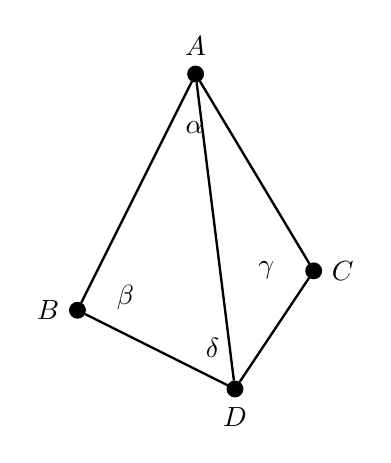
\begin{tikzpicture}[node distance=3cm]
                        \node[node, label=above:$A$](A) {};
                        \node[node, label=left:$B$,below of=A,xshift=-1.5cm](B) {};
                        \node[node, label=right:$C$,below of=A,xshift=1.5cm,yshift=0.5cm](C) {};
                        \node[node, label=below:$D$,below of=A,xshift=0.5cm,node distance=4cm](D) {};
            
                        \draw[-,line width=0.3mm](A) -- (B);
                        \draw[-,line width=0.3mm](A) -- (C);
                        \draw[-,line width=0.3mm](B) -- (D);
                        \draw[-,line width=0.3mm](C) -- (D);
                        \draw[-,line width=0.3mm](A) -- (D);
            
                        \centerarc[line width=0.1mm](A)(-60:-115:0.5);
                        \centerarc[line width=0.1mm](B)(65:-25:0.5);
                        \centerarc[line width=0.1mm](C)(-125:-240:0.5);
                        \centerarc[line width=0.1mm](D)(45:155:0.5);
            
                        \node[below left=4mm and -3mm of A,draw=none]() {$\alpha$};
                        \node[above right=-2mm and 3mm of B,draw=none]() {$\beta$};
                        \node[above left=-3mm and 3mm of C,draw=none]() {$\gamma$};
                        \node[above left=2mm and 0mm of D,draw=none]() {$\delta$};
                    \end{tikzpicture}
                    \subcaption{\centering Условие Делоне не выполнено $\beta+\gamma>180^\circ$}
                \end{subfigure}
                \begin{subfigure}{0.49\linewidth}
                    \centering
                    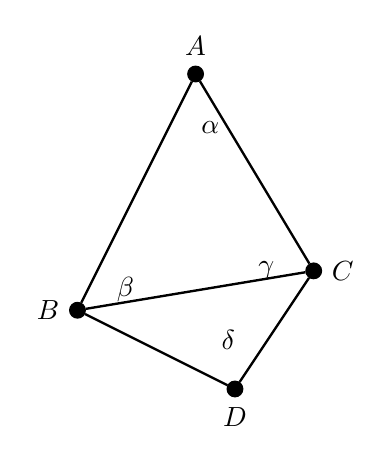
\begin{tikzpicture}[node distance=3cm]
                        \node[node, label=above:$A$](A) {};
                        \node[node, label=left:$B$,below of=A,xshift=-1.5cm](B) {};
                        \node[node, label=right:$C$,below of=A,xshift=1.5cm,yshift=0.5cm](C) {};
                        \node[node, label=below:$D$,below of=A,xshift=0.5cm,node distance=4cm](D) {};
            
                        \draw[-,line width=0.3mm](A) -- (B);
                        \draw[-,line width=0.3mm](A) -- (C);
                        \draw[-,line width=0.3mm](B) -- (D);
                        \draw[-,line width=0.3mm](C) -- (D);
                        \draw[-,line width=0.3mm](B) -- (C);
            
                        \centerarc[line width=0.1mm](A)(-60:-115:0.5);
                        \centerarc[line width=0.1mm](B)(65:-25:0.5);
                        \centerarc[line width=0.1mm](C)(-125:-240:0.5);
                        \centerarc[line width=0.1mm](D)(45:155:0.5);
            
                        \node[below left=4mm and -5mm of A,draw=none]() {$\alpha$};
                        \node[above right=-1mm and 3mm of B,draw=none]() {$\beta$};
                        \node[above left=-3mm and 3mm of C,draw=none]() {$\gamma$};
                        \node[above left=3mm and -2mm of D,draw=none]() {$\delta$};
                    \end{tikzpicture}
                    \subcaption{\centering Условие Делоне выполнено $\alpha+\delta\leqslant180^\circ$}
                \end{subfigure}
                \caption{\label{fig::flipping}Операция разворота ребра}
            \end{figure}
            Такой алгоритм не является наиболее эффективным, однако прост в реализации и показывает достаточную в рамках данной задачи производительность, время работы которого отображено в Таб. \ref{tbl::shull}.
            \begin{table}[h]
                \centering
                \begin{tabular}{|c|c|}
                    \hline
                    Количество точек & Время работы, мкс\\
                    \hline
                    $10$ & $50$\\
                    \hline
                    $10^2$ & $200$\\
                    \hline
                    $10^3$ & $5000$\\
                    \hline
                    $10^4$ & $50\cdot10^3$\\
                    \hline
                    $10^5$ & $48\cdot10^4$\\
                    \hline
                    $10^6$ & $7\cdot10^6$\\
                    \hline
                \end{tabular}
                \caption{\label{tbl::shull}Время работы алгоритма s-hull на случайно сгенерированных точках}
            \end{table}
            \newpage
            \par Для поиска треугольника, содержащего точку, был использован следующий алгоритм:
            \begin{enumerate}
                \item Обозначим $p$ --- искомая точка;
                \item Выберем случайный треугольник $t_0$ из триангуляции;
                \item \label{alg::3}Если точка принадлежит треугольнику, то алгоритм закончен;
                \item Иначе проведём отрезок $qp$, где $q$ --- некоторая внутрення точка треугольника, и найдём ребро $e$, пересекающее этот отрезок;
                \item Если ребро $e$ имеет соседа $t_1$, то обозначить $t_0=t_1$ и перейти к \ref{alg::3};
                \item Иначе алгоритм закончен.
            \end{enumerate}
    \section{Реализация и тестирование}
        \par В ходе работы было написано около 3000 строк кода на языке программирования C++, сделано 45 коммитов, разработана и реализована численная схема \ref{sec::numerical_scheme} решения уравнения \eqref{eq::WAMPE}, выполнена интеграция пакета Cambala для решения акустической спектральной задачи \eqref{eq::modal_equation}. Исходный код программы размещён в открытом доступе:
        \begin{itemize}
            \item \textsf{Acoustic}: \url{https://github.com/GoldFeniks/Acoustic}
            \item \textsf{delaunay}: \url{https://github.com/GoldFeniks/delaunay}
        \end{itemize}
        \par Тестирование проводилось путём проведения вычислительного эксперимента и сравнения его результатов с аналитическими решениями и другими известными методами.
        \subsection{Вычислительный эксперимент}
            \par Во время проведения вычислительных экспериментов коэффициенты $a$, $b$, $c$ в \eqref{eq::rational_linear} были выбраны из аппроксимации квадратного корня Клаербоута \cite{jensen}:
            \begin{equation}
                \sqrt{1+L_j}\simeq\frac{1+0.75L_j}{1+0.25L_j}\,.
            \end{equation}
            \subsubsection{Волновод мелкого моря с плоским дном}
                \par Проверка корректности работы численной схемы и условий прозрачной границы была проведена на примере моделирования распространения акустических волн в волноводе Пекериса, являющимся волноводом с постоянной глубиной дна, поэтому модовые функции и волновые числа зависят только от глубины. В рамках такой задачи известно аналитическое решение, которое может быть записано как \cite{jensen}
                \begin{equation}
                    \pa{x,y,z}=\frac{i}{4}\sum\limits_{j=1}^\infty\varphi_j\pa{z_s}\varphi_j\pa{z}H_0^{\pa{1}}\pa{k_j\sqrt{x^2+y^2}}\,,
                \end{equation}
                где $H_0^{\pa{1}}$ --- функция Ханкеля нулевого порядка первого рода \cite{hankel}. При проведении эксперимента были установлены следующие параметры:
                \begin{itemize}
                    \item Источник расположен на глубине $z_s=100\,\text{м.}$;
                    \item Глубина дна равна $200\,\text{м.}$;
                    \item Звуковое поле вычисляется на глубине $z=30\,\text{м.}$ на равномерной сетке:
                        \begin{equation}
                            \begin{aligned}
                                y_0&=-4\,\text{км.}\,,&y_1&=4\,\text{км.}\,,&M&=8001\,,\\
                                &&x_1&=10\text{км.}\,,&N&=10001\,.
                            \end{aligned}
                        \end{equation}
                \end{itemize}
                Время вычисления составило $13\,\text{с.}$
                \par Результат вычислений показан на Рис. \ref{fig::pekeris}. Из рисунка видно, что в основном численная схема корректно аппроксимирует аналитическое решение, хотя некоторый численный шум присутствует около источника. Также следует заметить, что несмотря на то, что уравнение является широкоугольным, оно всё ещё имеет ограниченную апертуру в горизонтальной плоскости. 
                \begin{figure}[h]
                    \centering
                    \begin{subfigure}[t]{\linewidth}
                        \centering
                        \includegraphics[width=0.49\linewidth]{pekeris_analytical}
                        \caption{Аналитическое решение}
                    \end{subfigure}
                    \begin{subfigure}[t]{0.49\linewidth}
                        \centering
                        \includegraphics[width=\linewidth]{pekeris_nampe}
                        \caption{Решение УМПУ}
                    \end{subfigure}
                    \begin{subfigure}[t]{0.49\linewidth}
                        \centering
                        \includegraphics[width=\linewidth]{pekeris_wampe}
                        \caption{Решение ШМПУ}
                    \end{subfigure}
                    \caption{\label{fig::pekeris}Акустическое поле (в дБ отн. 1 м.) в волноводе Пекериса на глубине $z=30\,\text{м.}$}
                \end{figure}
            \newpage
            \subsubsection{Мелкое море с подводным каньоном}
                \par Следующим численным экспериментом является моделирование распространения звуковых волн, создаваемых точечным источником в мелком море с подводным каньоном, схематическое изображение такого волновода изображено на Рис. \ref{fig::canyon}.
                \begin{figure}[h]
                    \centering
                    \includegraphics[scale=0.2]{canyon}
                    \caption{\label{fig::canyon}Схематическое изображение подводного каньона}
                \end{figure}
                Рельеф дна описывается функцией
                \begin{equation}
                    z=h\pa{y}=h_0+\Delta h\sec\pa{\sigma y}\,.
                \end{equation}
                Точечный источник $S$ расположен по координатам $x=y=0$, $z=z_s$.
                \newpage
                \par В данном численном эксперименте звуковое поле было вычислено на глубине $z=z_s$, и были использованы следующие параметры:
                \begin{equation}
                    \begin{aligned}
                        h_0&=50\,\text{м.}\,,&\Delta h&=5\,\text{м.}\,,&\sigma&=0.005\,,\\
                        z_s&=100\,\text{м.}\,,&x_1&=30\,\text{км.}\,,&N&=30001\,,\\
                        y_0&=-1\,\text{км.}\,,&y_1&=1\,\text{км.}\,,&M&=2001\,.
                    \end{aligned}
                \end{equation}
                Время вычисления составило $141\,\text{с.}$
                \par Результат вычислений показан на Рис. \ref{fig::TLfield}. Решение широкоугольного параболического уравнения сравнивается с так называемым узкоугольным адиабатическим МПУ \cite{jensen,petrov16}. Из Рис. \ref{fig::TLcomp} видно, что решения совпадают. Таким образом, разработанная численная схема хорошо подходит для моделирования распространения звука в волноводе мелкого моря с неоднородностями дна. Также этот результат показывает, что, апертуры узкоугольного МПУ достаточно для корректного решения данной задачи. Однако в общем случае известно, что узкоугольное уравнение недостаточно точно, так как горизонтальные лучи преломлённые неоднородностями дна могут распространяться под большими углами, которые не могут быть учтены такой аппроксимацией.
                \begin{figure}[H]
                    \centering
                    \includegraphics[width=0.49\linewidth]{TLfield}
                    \caption{\label{fig::TLfield}Акустическое поле (в дБ отн. 1 м) на глубине $z=10\,\text{м.}$ в волноводе мелкого моря с подводным каньоном}
                \end{figure}
                \begin{figure}[H]
                    \centering
                    \includegraphics[width=\linewidth]{TLcomp}
                    \caption{\label{fig::TLcomp}Сравнение результатов вычисления акустического поля (в дБ отн. 1 м) в мелком море с подводным каньоном вдоль оси $y=0$ на глубине $z=10\,\text{м.}$}
                \end{figure}
            \subsubsection{Мелкое море с подводным клином}
                \par В качестве последнего эксперимента было проведено моделирование распространения звуковых волн в мелком море с подводным клином. Схематичное изображения этого волновода изображено на Рис. \ref{fig::wedge}.
                \begin{figure}[h]
                    \centering
                    \includegraphics[width=0.49\linewidth]{wedge}
                    \caption{\label{fig::wedge}Схематичное изображение подводного клина}
                \end{figure}
                Рельеф дна описывается формулой:
                \begin{equation}
                    z=h\pa{y}=h_0+y\tan\alpha\,.
                \end{equation}
                \par Точечный источник расположен достаточно далеко от вершины клина на глубине $z=z_s$. Акустическое поле было вычислено на глубине $z_s=10\,\text{м.}$, и были использованы следующие параметры:
                \begin{equation}
                    \begin{aligned}
                        z_s&=100\,\text{м.}\,,&h_0&=200\,\text{м.}\,,&\alpha&\approx3.017^\circ\,,\\
                        &&x_1&=25\,\text{км.}\,,&N&=25001\,,\\
                        y_0&=-3.32\,\text{км.}\,,&y_1&=3.32\,\text{км.}\,,&M&=6641\,.
                    \end{aligned}
                \end{equation}
                Время вычисления составило $48\,\text{с.}$
                \par Результат вычисления показан на Рис. \ref{fig::wedge_field}, на котором видно, что так как используемая модель не учитывает модового взаимодействия, звуковое поле обрезается, ввиду того, что при уменьшении глубины дна пропадают моды старших порядков. Решение ШМПУ сравнивается с решением методом мнимых источников \cite{deane93,tang18} и УМПУ. Как показано на Рис. \ref{fig::wedge_comp}, решение ШМПУ почти совпадает с решением методом мнимых источников, при этом совпадение с УМПУ уменьшается при движении вдоль оси. Таким образом, в рамках данной задачи для получения корректного решения достаточно использовать широкоугольное модовое параболическое уравнение, а межмодовым взаимодействием можно пренебречь. 
                \begin{figure}[H]
                    \centering
                    \includegraphics[width=0.49\linewidth]{wedge_field}
                    \caption{\label{fig::wedge_field}Акустическое поле (в дБ отн. 1 м.) на глубине $z=30\,\text{м.}$ в волноводе мелкого моря с подводным каньоном}
                \end{figure}
                \begin{figure}[H]
                    \centering
                    \includegraphics[width=\linewidth]{wedge_comp}
                    \caption{\label{fig::wedge_comp}Сравнения результатов вычисления акустического поля (в дБ отн. 1 м.) в мелком море с подводным клином вдоль оси $y=0$ на глубине $z=30\,\text{м.}$}
                \end{figure}
        \subsection{Результаты вычислительного эксперимента}
            \par В результате вычислительного эксперимента было показано, что разработанная численная схема работает корректно и может быть использована при моделировании распространения звука в волноводах мелкого моря с неоднородностями дна. При этом ШМПУ применимо в большем множестве задач по сравнению с УМПУ. Также в некоторых задачах более вычислительно затратные методы могут быть заменены решением ШМПУ, вычисление которое требует гораздо меньше затрат.
    \section{Заключение}
        \par Таким образом в рамках проделанной работы были исследованы методы решения МПУ с применением условий прозрачной границы; разработана численная схема решения ШМПУ с использованием полностью дискретных условий прозрачной границы; разработан комплекс программ на языке C++, реализующий полученную численную схему и использующий пакет Cambala для решения акустической спектральной задачи; проведён вычислительный эксперимент, изучены корректность и область применения ШМПУ.
        \par Результаты работы были представлены на ежегодной международной конференции <<Дни Дифракции 2019>> \cite{dda} и будут опубликованы в научном издании Proceedings of International Conference <<Days on Diffraction 2019>>, индексируемом в Scopus/Web of Science \cite{dd}.
        \par В дальнейшем возможна разработка модели, учитывающей межмодовое взаимодействие и методов её решения.
        \par Все задачи, поставленные в ходе работы, выполнены успешно.
    \newpage
    \bibliographystyle{ugost2008ls}
    \bibliography{references.bib}	
    \glsaddall	
\end{document}
